\documentclass{article}

% Language setting
% Replace `english' with e.g. `spanish' to change the document language
\usepackage[english]{babel}

% Set page size and margins
% Replace `letterpaper' with `a4paper' for UK/EU standard size
\usepackage[letterpaper,top=2cm,bottom=2cm,left=3cm,right=3cm,marginparwidth=1.75cm]{geometry}

% Useful packages
\usepackage{amsmath}
\usepackage{amssymb}
\usepackage{graphicx}
\usepackage{inconsolata}
\usepackage{minted}
\usepackage[colorlinks=true, allcolors=blue]{hyperref}

\title{Innlevering 1: Del 6-8}
\author{Skrevet av André Hansen}

\begin{document}
\maketitle

\begin{abstract}
Dette er det løsning for første innlevering som dekker del 6-8 i pensum. Jeg kommer til å behandle denne innleverigen på lik linje som selve eksamenen.
\end{abstract}

\section{Uten hjelpemidler}

\subsection{Oppgave 1: I hvilket omløp og i hvilke kvadrant ligger vinkel $v= \frac{29 \pi}{9}$?}

vinkelen befinner seg i første kvadrant og er på sitt andre omløp

$$v = \frac{28 \pi}{9} = 2 \pi + \frac{\pi 10}{9}$$

\subsection{Oppgave 2: Oppgi de nøaktige verdiene}

\subsubsection{$tan 45^{\circ}$}

$$\tan 45^{\circ} = 1$$

\subsubsection{$sin 120^{\circ}$}

$$\sin 120^{\circ} = \frac{\sqrt{3}}{2}$$

\subsubsection{$cos 240^{\circ}$}

$$\cos 240^{\circ} = -\frac{1}{2}$$

\subsection{Oppgave 3:}

\subsubsection{Hva er komplemtnvinkelen til $52^{\circ}$}

Komplementvinkelen kan finnes ved å løse ligningen:

$$52^{\circ}+x^{\circ}=90^{\circ} \rightarrow x=38^{\circ}$$

Komplementvinken er $38^{\circ}$

\subsubsection{Hva er supplementvinkelen til $\frac{\pi}{5}$ , målt i grader?}

Supplementvinkelen kan finnes ved å løse ligningen:

$$\frac{\pi}{5} + x = \pi \rightarrow x = \pi - \frac{\pi}{5} \rightarrow x = \frac{4\pi}{5} = 144^\circ$$

Supplementvinkelen er $144^\circ$

\subsection{Oppgave 4: }

\subsubsection{$4(\sin x-\frac{3}{2}) = 2 \sin x-5, \quad x \in \mathbb{R}$}

\begin{align*}
    4(\sin x-\frac{3}{2}) &= 2\sin x-5, \quad x \in \mathbb{R} \\
    4\sin x - \frac{12}{2} &= 2 \sin x-5 \\
    2\sin x &= 1 \\
    \sin x &= \frac{1}{2} \\
    x &= \frac{\pi}{6} \cdot 2\pi \cdot k \lor x = \frac{5 \pi}{6} \cdot 2 \pi \cdot k , \quad k \in \mathbb{Z}
\end{align*}

\subsubsection{$\sqrt{2} \tan 2x = \sqrt{6}, \quad x \in [-\pi, \pi)$}

\begin{align*}
    \sqrt{2} \tan 2x &= \sqrt{6}, \quad x \in [-\pi, \pi) \\
    \tan 2x &= \sqrt3
\end{align*}

Generell løsning

\begin{align*}
    2x &= \frac{\pi}{3} + \pi \cdot k, \quad k \in \mathbb{Z} \\
    x &= \frac{\pi}{6} + \frac{\pi \cdot k}{2}
\end{align*}

Prøver med forskjellige verdier for $k$

\begin{align*}
    x &= \frac{\pi}{6} - \frac{\pi}{2}, \quad k = -2 \\
    x &= -\frac{5\pi}{6}
    \newline \\
    x &= \frac{\pi}{6} - \frac{\pi}{2}, \quad k = -1 \\
    x &= -\frac{\pi}{2}
    \newline \\
    x &= \frac{\pi}{6} + \frac{\pi \cdot k}{2}, \quad k = 0 \\
    x &= \frac{\pi}{6}
    \newline \\
    x &= \frac{\pi}{6} + \frac{\pi \cdot k}{2}, \quad k = 1 \\
    x &= \frac{2\pi}{3}
    \newline \\
\end{align*}

Så løsningen blir da:

$$ x \in \{ -\frac{5\pi}{6}, -\frac{\pi}{2}, \frac{\pi}{6} , \frac{2\pi}{3} \} $$

\subsubsection{$3 \sin(x + \frac{\pi}{12}) - \sqrt{3} \cos (x+\frac{\pi}{12})=0, \quad x\in\mathbb{R}$}

\begin{align*}
    3 \sin(x + \frac{\pi}{12}) - \sqrt{3} \cos (x+\frac{\pi}{12}) &= 0, \quad x\in\mathbb{R} \\
    \text{Omskriver til en sin funksjon på formen:} \\
    A \sin (x \cdot c+\phi) &= 0 \\
    A = \sqrt{3^2 - \sqrt{3}^2} &= 2 \cdot \sqrt{3} \\
    c &= 1 \\
    \tan \phi = \frac{\sqrt{3}}{3} \rightarrow \phi &= \frac{\pi}{6} \lor \frac{7\pi}{6} \\
    \text{ny formel} \\
    2\sqrt3 \sin (x+\frac{\pi}{6}) = 0 & \lor  2\sqrt{3} \sin (x+\frac{7\pi}{6}) = 0 \\
    \text{løsnig} \\
    \sin (x+\frac{\pi}{6}) = 0 & \lor \sin (x+\frac{7\pi}{6}) = 0 \\
    x+\frac{\pi}{6} = \frac{\pi}{2} + 2\pi \cdot k & \lor  x+\frac{7\pi}{6} = \frac{\pi}{2} + 2\pi \cdot k, \quad k\in\mathbb{Z} \\
    x = \frac{\pi}{3} + 2\pi \cdot k & \lor  x = -\frac{2\pi}{3} + 2\pi \cdot k, \quad k\in\mathbb{Z}
\end{align*}

\subsubsection{$ \cos 2x + \cos x = 0, \quad x\in[0, 2\pi)$}

\begin{align*}
    \cos 2x + \cos x &= 0, \quad x\in[0, 2\pi) \\
    \cos^2x - \sin^2x + \cos = 0 \\
    \cos^2x - (1-\cos^2x) \\
    x = 0
\end{align*}

\subsubsection{$\cos x - \sin x = \frac{\cos 2x}{\cos x + \sin x}$}

\begin{align*}
    \cos x - \sin x &= \frac{\cos 2x}{\cos x + \sin x} \\
    \cos x - \sin x &= \frac{\cos^2x - \sin^2x}{\cos x + \sin x} \\
    \frac{(\cos x - \sin x)(\cos x + \sin x)}{\cos x + \sin x} &= \frac{\cos^2x - \sin^2x}{\cos x + \sin x} \\
    \frac{\cos^2x - \sin^2x}{\cos x + \sin x} &= \frac{\cos^2x - \sin^2x}{\cos x + \sin x} \\
    0 &= 0 \\
    x &\in \mathbb{R} 
\end{align*}

\subsubsection{$\sin^2x = (1-\cos x)^2, \quad x \in [0, 2\pi)$}

\begin{align*}
    \sin^2x &= (1-\cos x)^2, \quad x \in [0, 2\pi) \\
    \sqrt{\sin x}^2 &= \sqrt{1-\cos x}^2 \\
    \sin x &= 1 - \cos x \\
    \sin x + \cos x &= 1 \\
    x = \frac{\pi}{2} + 2\pi \cdot k & \lor  x = 2\pi \cdot k,\quad k \in \mathbb{Z} \\
    x = 2\pi \cdot k &, \quad k \in \mathbb{Z} \quad \text{har ingen løsninger} \\
    x = \frac{\pi}{2}
\end{align*}

\subsection{Oppgave 5: Gitt funksjonen $f(x)=2sin(\frac{x}{2}+\frac{\pi}{4})-1, \quad x \in [-4\pi, 4\pi)$}

\subsubsection{hva er nullpunktene til $f(x)$}

\begin{align*}
    f(x) &= 0 \\
    2\sin(\frac{x}{2}+\frac{\pi}{4})-1 &= 0 , \quad x \in [-4\pi, 4\pi)  \\
    2\sin(\frac{x}{2}+\frac{\pi}{4}) &= 1 \\
    \sin(\frac{x}{2}+\frac{\pi}{4}) &= \frac{1}{2} \\
    \frac{x}{2} + \frac{\pi}{4} = \frac{\pi}{6} + 2\pi \cdot k  & \lor \frac{x}{2} + \frac{\pi}{2} = \frac{\pi}{6} \cdot 2\pi \cdot k, \quad k\in\mathbb{Z} \\
    x+\pi=\frac{\pi}{3} + 4\pi \cdot k &\lor x + \pi = \frac{\pi}{3} + 4\pi \cdot k \\
    x=-\frac{2\pi}{3} \cdot 4\pi \cdot k & \lor  x=\frac{4\pi}{3} + 4\pi \cdot k \\
    x=-\frac{2\pi}{3} + 4\pi \cdot k & \lor  x=\frac{4\pi}{3} + 4\pi \cdot k, \quad k \in \{ -1, 0, 1\} \\
    L= \{-\frac{8\pi}{3}, -\frac{2\pi}{3}, & \frac{4\pi}{3}, \frac{10\pi}{3} \}
\end{align*}

\subsubsection{Skiser grafen}

\begin{figure}[h]
    \centering
    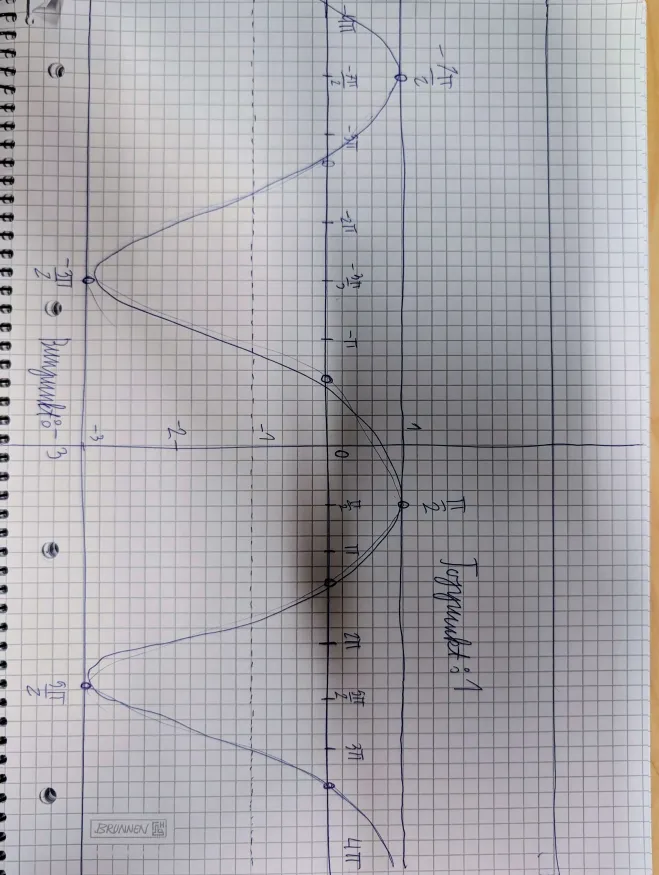
\includegraphics[width=0.7\textwidth, angle=90]{tegning.png}
    \caption{Skisse av grafen}
\end{figure}

\subsection{Oppgave 6: Deriver funksjoneen}

\subsubsection{$f(x)=x^3 \cdot \sin x$}

\begin{align*}
    f'(x) &= [x^3]' \cdot \sin x + x^3 \cdot [\sin x]' \\
    &= 3x^2 \cdot \sin x + x^3 \cdot \cos x \\
    &= x^2(3 \sin x - x \cos x)
\end{align*}

\subsubsection{$g(x)=\frac{1}{2} \cos(2x^2)$}

\begin{align*}
    g(x)'&=[\frac{1}{2} \cos(2x^2)]' \\
    &=[\frac{1}{2}]'\cdot\cos(2x^2) + \frac{1}{2}\cdot[\cos(2x^2)] \\
    &= \frac{1}{2} \cdot [\cos(2x^2)]' \\
    &= \frac{1}{2} \cdot -\sin(2x^2) \cdot 4x \\
    &= -2x\sin(2x^2)
\end{align*}

\subsection{Oppgave 7: Regn ut integralene}

\subsubsection{$\int_{\frac{\pi}{3}}^{\pi}(\sin x + \cos x) \, dx$}

\begin{align*}
    \int_{\frac{\pi}{3}}^{\pi}(\sin x + \cos x) \, dx \\
    &= [\sin x - \cos x]^\pi_\frac{\pi}{3} \\
    &= \sin(\pi) - \cos(\pi) - (\sin(\frac{\pi}{3}) - \cos (\frac{\pi}{3})) \\
    &= \sin(\pi)-\sin(\frac{\pi}{3})-\cos (\pi) - \cos (\frac{\pi}{3}) \\
    &= 1 - \frac{\sqrt{3}}{2} + \frac{1}{2} \\
    &= \frac{3-\sqrt{3}}{2}
\end{align*}

\subsubsection{$\int (x \cdot \sin 2x)dx$}

\begin{align*}
    \text{Bruker: } \int u' \cdot v \, dx = u \cdot v &- \int u \cdot v' \, dx \quad \text{setter $x=v$ og $\sin 2x = u'$} \\
    \int (x \cdot \sin 2x) \, dx &= x \int \sin 2x \, dx - \int (x' \cdot \int \sin 2x \, dx) \, dx\\
    &= x \int \sin 2x \, dx - \iint \sin 2x \, dx\\
    &= 2x \int \sin x \cos x \, dx - \int 2 \int \sin x \cos x \, dx \, dx \\
    &= 2x \int \sin x \cos x - 2 \iint \sin x \cos x \, dx \, dx \\
    &= \text{Det var så mye jeg klarte...}
\end{align*}

\section{Del 2: Med hjelpemidler}

\subsection{Oppgave 8: Et fly har resit 26,0 km. Finn lengden nord}

$\sin(41^{\circ} \cdot 26,0km) \approx 19.32 km$

\text{Flyet har reist ca $19,32km$ nord}

\subsection{Oppgave 9: Finn høyden av tårnet}

\text{Høyden av tårned kan finnes ved å definere to funksjoner for hver av vinkelene og finne kjæringspunktet}

\begin{align*}
    f(x) &= x\tan(16.7^\circ) \quad g(x)=(x-85.3)\tan(21.4^\circ) \\
    \text{Løser:} \\
    f(x) &= h(x) \\
    x &\approx 363.82 \\
    h \approx f(363.82) \approx 109.15 
\end{align*}

\text{Høyden til tårnet er ca $109.15m$}

\subsection{Oppgave 10: }

\subsubsection{Bruk formelene for sinus og cosinus til en differanse mellom to vinkler til å vise at $\tan(u-v)=\frac{\tan u-\tan v}{1+\tan u \tan v}$}

\text{Formelene til sinus og cosinus sier:}

\begin{align*}
    sin(u-v) &= \sin u\cos v - \sin v \cos u  \\
    cos(u-v) &= \cos u\cos v +\sin u \sin v
\end{align*}

\begin{align*}
    \tan(u-v) &= \frac{\sin u-v}{\cos u-v} \\
    &= \frac{\sin u \cos v - \sin v \cos u}{\cos u \cos v + \sin u \sin v} \\
    & \text{Deler nevner og teller på:} \cos u \cos v \\
    &= \frac{\frac{\sin u \cos v}{\cos u \cos v} - \frac{\sin v \cos u}{\cos v \cos u}}{\frac{\cos u \cos v}{\cos u \cos v} + \frac{\sin u \sin v}{\cos u \cos v}} \\
    &= \frac{\frac{\sin u \cos v}{\cos u \cos v} - \frac{\sin v \cos u}{\cos v \cos u}}{1 + \frac{\sin u \cos v}{\cos u \cos v} \cdot \frac{\sin v \cos u}{\cos u \cos v}} \\
    &= \frac{\frac{\sin u}{\cos u} - \frac{\sin v}{\cos v}}{1 + \frac{\sin u }{\cos u } \cdot \frac{\sin v}{\cos v}} \\
    &= \frac{\tan u - \tan v}{1 + \tan u \tan v}
\end{align*}

\subsubsection{Skriv $\sin 3x$ utrykt ved $\sin x$}

\begin{align*}
    \sin(3x) &= \sin(2x+x) \\
    &= \sin 2x \cos x +\sin x \cos 2x \\
    &= 2 \sin x \cos^2x + (\cos^2x - \sin^2x)\sin x \\
    &= 2 \sin x (1-\sin^2x) + ((1-\sin^2x)-\sin^2x)\sin x \\
    &= 2 \sin x - 2 \sin^3x + \sin x - 2 \sin^3x \\
    &= 3 \sin x - 4 \sin^3x
\end{align*}

\subsection{Opgpave 11: }

\subsubsection{Lag linære modeller f(x) og g(x) for henholdsvis antall bensinbiler og antall elbiler i Norge, der x er antall år etter 1.1.2016}

Ved regresjonsanalyse i geogebra får man:

\begin{align*}
    f(x)=-60082.2x + 1198697.6 \\
    h(x)=60664.9 + 85182.2 \\
\end{align*}

\subsubsection{Hvis vi antar at modellene er gyldige noen år framover, i hvilket år vil vi for første gang ha flere elbiler enn bensinbiler i Norge?}

\begin{align*}
    g(x)=h(x) \\
    x \approx 9.22 \\
    \text{i løpet av det niende året vil det være flere elbiler en bensinbiler}
\end{align*}

\subsection{Oppgave 12:}  

\subsubsection{Lag en modell $f(x)$ for befolknings årlige vekstfart}

\text{Modellen etter regersjonsanalyse som polynomfunksjon er:}

$$g(x)=287.87x^2-4380.35x + 30391.35$$

\subsubsection{Hvor mange innbyggere var det i Norge $1.1.1976$ ifølge modellen?}

\text{Først defineres en funksjon for befolkningsvekst ved å løse differensialigningen:}

$$y' = g(x)$$

\text{Dette gir at befolkningsveksten $f(x)=95.96x^3-2190.17x^2+30391.35x+3917773$}

$$f(4)\approx4010437$$

\subsubsection{Hvilket år passerte folketallet 4,2 millioner ifølge modellen?}

$f(x)=0 \rightarrow x=14.84$

\text{Ifølge funksjonen passerer folketallet $4,2$ 14.84 år etter 1972}

\subsection{Oppgave 13: En fabrikk sliper ved uhel 500 kg gift i et tjern som inneholder $2\cdot 10^10$ liter vann. Hver time renner det ut og inn $10^7$}

\text{Giften i tjernet kan moduleres ved å bruke differensialigningen :} $y'= \frac{-y \cdot 10^7}{2 \cdot 10^{10}}, \quad y(0) = 500$

\text{Løsningen CAS gir er : }

\begin{align*}
    y = 500 \cdot e^{\frac{-x}{2000}} = f(x) \\
    f(x) = 100 \\
    x \approx 3219 timer \\
    3219 \, timer \div 24 \, timer \approx 129 \, dager
\end{align*}

\text{det vil ta ca $129$ dager før giften er redusert til $100$ kg}

\bibliographystyle{alpha}
\bibliography{sample}

\end{document}
